\documentclass[11pt]{article}

\usepackage[a4paper,margin=1in]{geometry}
\usepackage{microtype}
\usepackage{amsmath,amssymb,amsfonts}
\usepackage{hyperref}
\usepackage{float}
\usepackage{placeins}
\usepackage{amsmath}
\usepackage{booktabs} 
\usepackage{array,booktabs,tabularx}
\usepackage{tikz}
\usetikzlibrary{arrows.meta,calc,angles,quotes}

 \newcolumntype{L}{>{\raggedright\arraybackslash}X}
 \newcommand{\sech}{\operatorname{sech}}


\numberwithin{equation}{section}

\title{Unimetry: A Phase-Space Reformulation of Special Relativity}
\author{Timur Abizgeldin\\ \small Independent researcher, Austria\\ \small \texttt{timurabizgeldin@gmail.com}}
\date{\today}


% --- Unimetry macros ---
\usepackage{tikz}
\usetikzlibrary{arrows.meta,positioning,calc}
\providecommand{\bi}{\mathbf{i}}
\providecommand{\bj}{\mathbf{j}}
\providecommand{\bk}{\mathbf{k}}
\providecommand{\uhat}{\hat{\mathbf u}}
\providecommand{\rotor}[2]{cos\frac{#2}{2} + #1\,sin\frac{#2}{2}}


\usepackage[nameinlink,capitalize,noabbrev]{cleveref}
\crefname{figure}{Fig.}{Figs.}
\Crefname{figure}{Fig.}{Figs.}
\crefname{table}{Table}{Tables}
\Crefname{table}{Table}{Tables}
\crefname{equation}{Eq.}{Eqs.}
\Crefname{equation}{Eq.}{Eqs.}
\crefname{section}{Sec.}{Secs.}
\Crefname{section}{Sec.}{Secs.}
\crefname{appendix}{App.}{Apps.}
\Crefname{appendix}{App.}{Apps.}
\begin{document}


% =============================================================
\section[Chapter 1. Flow]{Chapter 1. Flow}
\label{ch:flow}
\textbf{Scope.} We introduce the flow model and define phase as its measure. We recall quaternions, state why we use them, and explain when a complex slice is used. We then introduce three angles—intrinsic ($\zeta$), gravitational ($\phi$), and kinematic ($\vartheta$)—and state the SR simplification.

\subsection[1.1. The spatially-linked quaternion]{1.1. The spatially-linked quaternion}
\label{subsec:spatialq}
Let $q(\mathbf x,t)\in S^3\simeq SU(2)$ denote the flow state. Fix an \emph{internal} imaginary basis $\{I,J,K\}\subset\Im\mathbb H$. The observed (lab) orthonormal triad is the conjugated image
\begin{equation}
\mathbf e_I(q)=q I q^{-1},\qquad \mathbf e_J(q)=q J q^{-1},\qquad \mathbf e_K(q)=q K q^{-1}.
\end{equation}
The \emph{time fiber} is generated by right multiplication with $e^{\frac{\phi}{2}K}$; its spatial director (shadow) is $\mathbf n(q)=qKq^{-1}\in S^2$.

\subsection[1.2. Why quaternion algebra]{1.2. Why quaternion algebra}
\label{subsec-1-2-why-quaternion-algebra}

Quaternions form the minimal non-commutative algebra that: (i) double-covers $SO(3)$ for rigid 3D rotations; (ii) carries the Hopf fibration $S^3\to S^2$, separating an internal S$^1$ time fiber from spatial orientations; and (iii) encodes non-commutativity necessary for Wigner--Thomas rotations (residual spatial rotations from composing non-collinear boosts). (Hopf~\cite{Hopf1931}; Wigner~\cite{Wigner1939}; Thomas~\cite{Thomas1926}).

\subsection[1.3. Why (and where) we use a complex slice]{1.3. Why (and where) we use a complex slice}
\label{subsec-1-3-why-and-where-we-use-a-complex-slice}

For exposition we sometimes restrict to the commuting slice $\mathrm{span}\{1,K\}\cong\mathbb C$, which preserves the time fiber while suppressing transverse components. We use this slice in SR derivations and in phase-1-form preliminaries; non-collinear compositions revert to the full quaternionic picture.

\subsection[1.4. Three angles]{1.4. Three angles}
\label{subsec:three-angles}
We introduce three angles with distinct roles:
\begin{itemize}
  \item \textbf{Intrinsic tilt} $\zeta\in[0,\tfrac{\pi}{2}]$: angle between the flow tangent and the time fiber. It controls optical and evolutionary (``Friedmann-like'') effects of the same flow:
  \begin{equation}
    v_{\rm ph}=ccos\zeta,\qquad n(\zeta)=\frac{c}{v_{\rm ph}}=\sec\zeta,\qquad \frac{d\tau}{dt}=cos\zeta.
  \end{equation}
  \item \textbf{Gravitational angle} $\phi$: an \emph{external} flow-induced tilt field. In the weak, stationary regime it encodes Schwarzschild-like clock and light effects via an effective index $n_g=\sec\phi$ and time-rate $d\tau/dt=\cos\phi$. We do not build full field equations here.
  \item \textbf{Kinematic angle} $\vartheta$: SR angle for relative motion between comoving flows:
  \begin{equation}
    \beta=sin\vartheta,\qquad \gamma=\sec\vartheta,\qquad \tanh\eta=sin\vartheta.
  \end{equation}
\end{itemize}

\subsection[1.5. SR simplification]{1.5. SR simplification}
\label{subsec-1-5-sr-simplification}

Whenever two objects share $\zeta_A=\zeta_B$ and $\phi_A=\phi_B$ along a worldline segment, a local comoving frame exists where SR applies. In SR-focused chapters we adopt $\zeta=\phi=0$ and retain only the kinematic angle $\vartheta$.


% =============================================================
\section[Chapter 2. The kinematic angle]{Chapter 2. The kinematic angle}
\label{ch:kin-angle}
\subsection[2.1. Definition]{2.1. Definition}
\label{subsec-2-1-definition}

Define $\vartheta$ so that SR kinematics lives on a circle rather than a hyperbola:
\begin{equation}
\beta=sin\vartheta,\qquad \gamma=\sec\vartheta,\qquad \tanh\eta=sin\vartheta,\qquad cosh\eta=\sec\vartheta.
\end{equation}

\subsection[2.2. Mapping and correspondence]{2.2. Mapping and correspondence}
\label{subsec-2-2-mapping-and-correspondence}

 oindent\textit{See also \Cref{fig:circle-hyperbola-gd}.}

\begin{table}[h]
  \centering
  \begin{tabular}{lll}\hline
    Quantity & Standard SR (hyperbolic) & Phase picture (circular) \\\hline
    Rapidity & $\eta$ & $\tanh\eta=\sin\vartheta$ \\
    Lorentz factor & $\gamma=\cosh\eta$ & $\gamma=\sec\vartheta$ \\
    Speed & $\beta=\tanh\eta$ & $\beta=\sin\vartheta$ \\
    Longitudinal Doppler & $k=e^{\pm\eta}$ & $k=\dfrac{1+\tan(\vartheta/2)}{1-\tan(\vartheta/2)}$ \\
    Temporal projection & $\sech\eta$ & $\cos\vartheta$ \\\hline
  \end{tabular}
  \caption{SR--phase correspondences for the kinematic angle.}
  \label{tab:sr-phase}
\end{table}

% Preserved figure from original manuscript:
\begin{figure}[!ht]
\centering
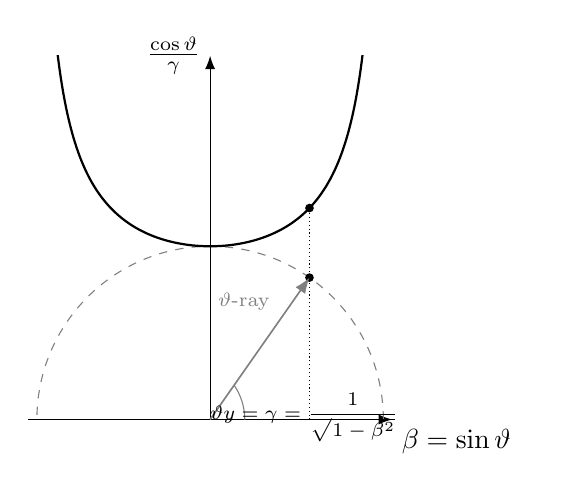
\begin{tikzpicture}[scale=2.2, >=Latex]
  % общие параметры
  \def\ymax{2.1}
  \def\th{35} % пример угла
  \pgfmathsetmacro{\bet}{sin(\th)}   % β = sin θ
  \pgfmathsetmacro{\co}{cos(\th)}    % cos θ
  \pgfmathsetmacro{\ga}{1/\co}       % γ = sec θ

  % оси (вне clip, чтобы надписи не резались)
  \draw[->] (-1.05,0) -- (1.05,0) node[below right] {$\beta=\sin\vartheta$};
  \draw[->] (0,0) -- (0,\ymax) node[left] {$\frac{\cos\vartheta}{ \gamma}$};

  \begin{scope}
    \clip (-1.05,0) rectangle (1.95,\ymax);

    \draw[gray,dashed] (0,0) circle (1);

    \draw[line width=0.8pt] plot[domain=-0.90:0.90, samples=240] (\x, {1/sqrt(1-\x*\x)});

    \draw[densely dotted] (\bet,0) -- (\bet,\ga);
    \fill (\bet,\co) circle (0.025);
    \fill (\bet,\ga) circle (0.025);
  \end{scope}

  \draw[gray,->,line width=0.6pt] (0,0) -- (\bet,\co) node[pos=0.7, above left] {\scriptsize $\vartheta$-ray};
  \draw[gray] (0.20,0) arc[start angle=0, end angle=\th, radius=\th/100];
   ode[gray] at (0.27,0.08) {\scriptsize $\vartheta$};

   ode[gray] at (-0.52,0.18) {\scriptsize phase circle};
   ode at (1.36,1.45) {\scriptsize $y=\gamma=\dfrac{1}{\sqrt{1-\beta^{2}}}$};
\end{tikzpicture}
\caption[Phase circle vs. Lorentz hyperbola at common . Vertical mapping at fixed illustrates the Gudermann bridge: .]{Phase circle vs. Lorentz hyperbola at common $\beta=\sin\vartheta$. Vertical mapping at fixed $\beta$ illustrates the Gudermann bridge: $\gamma=\sec\vartheta=\cosh\eta$. See mapping in \cref{tab:sr-phase}.}
\label{fig:circle-hyperbola-gd}
\end{figure}
\FloatBarrier

\section[Time and space as phase derivatives]{Time and space as phase derivatives}
\label{sec-time-and-space-as-phase-derivatives}


\paragraph{Why a complex slice of a quaternion?}
For local kinematics any unit direction $\uhat$ singles out the two--dimensional subalgebra
$\mathrm{Span}\{1,\uhat\}\cong\mathbb{C}\subset\mathbb{H}$. Working in this complex
\emph{slice} preserves all boost/rotation algebra along $\uhat$, but keeps formulas
elementary. When the direction changes, one updates the slice; the full quaternionic
structure is retained.

Let $\vec{\chi}\in\mathbb{C}$ be a variable whose change generates observable time-space effects. We treat the time and space units as directional derivatives (phase velocities) along the real and imaginary directions of a complex basis $(\hat{h},\mathbf{l})$:
\begin{equation}
\hat{h}\,dx_0=\frac{\partial\vec{\chi}}{\partial\chi_h}\frac{d\chi_h}{d\chi}\,d\chi
=\tilde{H}\,d\chi,\qquad
\mathbf{l}\,dx_l=\frac{\partial\vec{\chi}}{\partial\chi_l}\frac{d\chi_l}{d\chi}\,d\chi
=\tilde{L}\,d\chi,\quad l=1,2,3.
\label{eq:11}
\end{equation}
Introduce the phase speed of the SR interval $ds=\tilde{S}\,d\chi$. The interval conservation takes the form
\begin{equation}
\tilde{S}^2=\frac{ds^2}{d\chi^2}
=\frac{g_{ij}\,dx^i dx^j}{d\chi^2}
=\left( \frac{\mathtt{c}^2 dt^2}{d\chi^2} \right) - \left[ \frac{\mathbf{dx}^2}{d\chi^2} \right]
=\left( \tilde{H}^2 \right) - \left[ \tilde{L}^2 \right],
\label{eq:12}
\end{equation}
equivalently
\begin{equation}
\tilde{H}^2=\tilde{S}^2+\tilde{L}^2.
\label{eq:13}
\end{equation}
Writing 
\begin{equation}
\tilde{S}=\tilde{H}cos\theta,\qquad \tilde{L}=\tilde{H}sin\theta,
\label{eq:14}
\end{equation}
where $\theta$ is the angle of the phase speed relative to the real axis. Algebraically, \eqref{eq:13} is a Euclidean decomposition of a single speed into orthogonal projections; physically, we will see that under reparameterization the \emph{projection} $\tilde{S}$, not the Euclidean norm $\tilde{H}$, is the conserved Minkowski quantity.

% --- patch: Flow and phase 1-form ---
\paragraph{Flow and phase 1-form.}
Let $\Phi:\mathcal E\to\mathbb R$ be a scalar \emph{phase potential} on a (possibly infinite-dimensional) Euclidean/Hilbert proto-space $(\mathcal E,\langle\cdot,\cdot\rangle)$. 
Define the phase 1-form $\alpha:=d\Phi$ and the associated \emph{flow vector} $\boldsymbol\chi:= abla\Phi$, where the gradient is taken with respect to $\langle\cdot,\cdot\rangle$.

Fix an observer's orthonormal spatial triad $\{\mathbf e_1,\mathbf e_2,\mathbf e_3\}\subset\mathcal E$ and let $S=\mathrm{span}\{\mathbf e_1,\mathbf e_2,\mathbf e_3\}$ with orthogonal projectors $P_S$ and $P_{S^\perp}$. 
Decompose
\[
\boldsymbol\chi=\boldsymbol\chi_S+\boldsymbol\chi_\perp,\qquad
\boldsymbol\chi_S:=P_S\boldsymbol\chi,\quad 
\boldsymbol\chi_\perp:=P_{S^\perp}\boldsymbol\chi.
\]
Define observable spatial components and the orthogonal magnitude
\[
\ell_i:=\langle\boldsymbol\chi,\mathbf e_i\rangle,\qquad 
\mathbf l:=\sum_{i=1}^3 \ell_i\,\mathbf e_i,\qquad 
t:=\|\boldsymbol\chi_\perp\|=\sqrt{\|\boldsymbol\chi\|^2-\|\boldsymbol\chi_S\|^2},
\]
and, for orientation when $t>0$, the unit direction $\mathbf e_t:=\boldsymbol\chi_\perp/\|\boldsymbol\chi_\perp\|$.
Then the phase angle $\vartheta$ and the direction $\mathbf u$ used throughout this paper are recovered as
\[
\cos\vartheta=\frac{t}{\|\boldsymbol\chi\|},\qquad 
\sin\vartheta=\frac{\|\mathbf l\|}{\|\boldsymbol\chi\|},\qquad 
\mathbf u=\frac{\mathbf l}{\|\mathbf l\|}\quad(\|\mathbf l\|>0).
\]
This complements the operational definition \eqref{eq:operational-phase} and ties the phase picture to a differential-form language.


\section[Phase space]{Phase space}
\label{sec-phase-space}

Let the phase vector space be $\mathbb{H}$ with orthonormal basis $(\hat{h},\mathbf{l})$. For a phase vector $\vec{\chi}=R\,e^{\theta\mathbf{l}}$ with $\theta\in[-\pi,\pi]$,
\begin{equation}
\tilde{H}=R,\qquad \tilde{S}=Rcos\theta,\qquad \tilde{L}=R\,\mathbf{l}sin\theta.
\label{eq:21}
\end{equation}
Choosing coordinates where the projectors onto $(\hat{h},\mathbf{l})$ are unit, \eqref{eq:11} simplifies to
\begin{equation}
\hat{h}\,dx_0=\frac{d\chi_h}{d\chi}\,d\chi=\tilde{H}\,d\chi,\qquad
\mathbf{l}\,dx_l=\frac{d\chi_l}{d\chi}\,d\chi=\tilde{L}\,d\chi.
\label{eq:22}
\end{equation}
The map from phase to observables is an integral transform:
\begin{equation}
x^i(\chi)=x^i(\chi_0)+\int_{\chi_0}^{\chi}\tilde{X}^i(u)\,du,\qquad i=0,1,2,3,
\label{eq:23}
\end{equation}
where $\tilde{X}^i$ are projections of $d\vec{\chi}/d\chi$ onto $(\hat{h},\mathbf{l})$ and $x^i(\chi_0)$ fix initial conditions.

\section[Objects]{Objects}
\label{sec-objects}

 oindent\textit{Roadmap.} The next formulas fix notation and the geometric carriers we use throughout. 
In particular, the phase state $(\vartheta,\mathbf u)$ selects a complex slice 
$\mathbb C_{\mathbf u}\subset\mathbb H$; collinear compositions become ordinary circular sums on this slice, 
while non-collinear compositions generate a genuine 3D rotation (Wigner–Thomas) via quaternion multiplication.
This explains why we keep both $\vartheta$ and $\mathbf u$ as primary objects.

A fundamental particle is an elementary object with nonzero phase $\vec{\chi} eq0$. Composite objects are phase configurations; to represent them in phase space one may require additional dimensions, except for the photon, whose phase is always aligned with the imaginary axis:
\begin{equation}
\mathbf{p}=\frac{d\vec{\chi}}{d\chi_l}=p\,\mathbf{l}\in\Im.
\label{eq:31}
\end{equation}
Non-photonic phenomena are associated with nonzero real projection and nonzero mass. A complex object can be identified with an event or worldline; the photon corresponds to a null-interval point encoding information about the event.

Any object's phase can be rotated to the \emph{zero} (purely real) direction,
\begin{equation}
\vec{\chi}_0=R\in\Re.
\label{eq:32}
\end{equation}
An object $A$ moving with speed $v$ relative to a rest observer has
\begin{equation}
\vec{\chi}_A=R\,e^{\vartheta_A\mathbf{l}},\qquad
sin\vartheta_A=\frac{v}{\mathtt{c}}\equiv\beta.
\label{eq:33}
\end{equation}

 oindent\textit{From unit norm to the interval.}
We will repeatedly use that $cd\tau= c\,dt\,\cos\vartheta$ and $d\mathbf x=c\,dt\,\sin\vartheta\,\mathbf u$.
Thus the identity $\cos^{2}\vartheta+\sin^{2}\vartheta=1$ is exactly the Minkowski metric statement 
$(cd\tau)^{2}=(cdt)^{2}-d\mathbf x^{2}$; from now on, square-root expressions are traded for circular 
trigonometry in $\vartheta$.


\subsection[Space as a symmetric phase pair]{Space as a symmetric phase pair}
\label{subsec-space-as-a-symmetric-phase-pair}

From \eqref{eq:14}, a naive zero-angle limit would remove the imaginary projection, contradicting observability. We enforce a nonvanishing spatial projection by pairing opposite-phase tilts:
\begin{equation}
\vec{\chi}^{\pm}=R\,e^{\pm\zeta\,\mathbf{l}},\qquad
\vec{\chi}_l:=\frac{\vec{\chi}^+-\vec{\chi}^-}{2}=R\,\mathbf{l}sin\zeta,
\label{eq:311}
\end{equation}
where $\zeta$ is an \emph{internal angle} (intrinsic to the object; heuristically linked to mass/density). The local decomposition is
\begin{equation}
\vec{\chi}_0=\vec{\chi}_\tau+\vec{\chi}_l
=Rcos\zeta+R\,\mathbf{l}sin\zeta,
\label{eq:312}
\end{equation}
with unit components (normalized by $R$): the real component is $\cos\zeta$ and the imaginary component is $\sin\zeta$.

\subsection[Absolute, local, and observed time]{Absolute, local, and observed time}
\label{subsec-absolute-local-and-observed-time}

Define \emph{absolute} time $t=t(\tilde{H})$ at the zero phase direction; it is the fastest clock and useful for normalization between different phase speeds. Along the local real direction,
\begin{equation}
dx_0=\frac{d}{d\chi}\Re(\vec{\chi})\,d\chi
=\frac{\vec{\chi}^+ + \vec{\chi}^-}{2}\,d\chi
=cos\zeta\,d\chi
=:d\tau.
\label{eq:321}
\end{equation}
Here $d\chi_0:=\cos\zeta\,d\chi$ is the projection of $d\chi$ onto the local real axis; in \cref{sec:norm} we calibrate $d\tau=(1/ u_0)\,d\chi_0$. The observed proper time of $A$ relative to the rest observer is
\begin{equation}
\tilde{H}_A=\Re\!\left(\frac{d\vec{\chi}_A}{d\vec{\chi}_0}\right)
=cos\vartheta_A
=\sqrt{1-sin^2\vartheta_A}
=\sqrt{1-\frac{v^2}{\mathtt{c}^2}}
=\frac{1}{\gamma}.
\label{eq:322}
\end{equation}

\subsection[Normalization]{Normalization}\label{sec:norm}
 oindent\textit{Calibration.}
We fix the calibration by the observer’s clock and speed budget: 
$\cos\vartheta \equiv d\tau/dt$ and $\sin\vartheta \equiv \beta$.
This choice does not restrict generality: any overall rescaling of the underlying flow is absorbed into the 
definitions of $t$ and $c$, leaving all dimensionless observables unchanged.

Let local time be parameterized by \emph{phase}; introduce a reference frequency $ u_0$ and set
\begin{equation}
d\tau=\frac{1}{ u_0}\,d\chi_0.
\label{eq:331}
\end{equation}
By the chain rule,
\begin{equation}
dx_0=\tilde{H}\,d\chi
=\frac{dx_0}{d\chi_0}\frac{d\chi_0}{d\tau}\,d\tau
=\tilde{H}\,\dot{\chi}\,d\tau
=: \dot{H}\,d\tau,
\label{eq:332}
\end{equation}
where $ u:=d\chi/d\tau$, $\dot{\chi}:= u/ u_0$, and $\dot{H}:=\tilde{H}\,\dot{\chi}$. Choosing the calibration $\dot{H}\equiv \mathtt{c}$ gives $dx_0=\mathtt{c}\,d\tau$. Similarly for space,
\begin{equation}
dx_l=\tilde{L}\,d\chi
=\frac{dx_l}{d\chi_0}\frac{d\chi_0}{dl}\,dl
=\tilde{L}\,\chi'\,dl
=:L'\,dl,\qquad \chi':=\frac{d\chi}{dl}.
\label{eq:333}
\end{equation}
From $dx_0=dx_l$ for light one gets
\begin{equation}
\mathtt{c}=\tilde{L}'\,\frac{dl}{d\tau},
\label{eq:334}
\end{equation}
hence with temporal calibration to $\mathtt{c}$ the spatial scale becomes unit: $\tilde{L}'=1$.

\subsection[Light and $c]{Light and $\mathtt{c}$ as a calibration constant}
From the normalized forms,
\begin{equation}
\frac{\mathtt{c}}{\dot{\chi}}\,d\chi=\frac{1}{\chi'}\,d\chi
\quad\Rightarrow\quad
\mathtt{c}=\frac{\dot{\chi}}{\chi'}=\frac{dl}{d\tau},
\label{eq:341}
\end{equation}
i.e.\ $\mathtt{c}$ is a \emph{calibration constant} tying temporal and spatial measures, independent of local phase variation. Equation \eqref{eq:341} also reads
\begin{equation}
\mathtt{c}=\left(\frac{d\chi}{d\tau}\right)\!\left[\frac{dl}{d\chi}\right]\sim ( u)\,[\lambda],
\label{eq:343}
\end{equation}
matching frequency and wavelength of a photon, with $\chi$ as its phase. For a lightlike trajectory,
\begin{equation}
ds^2=\mathtt{c}^2\!\left(\frac{d\chi^2}{\dot{\chi}^2}-\frac{d\chi^2}{\dot{\chi}^2}\right)=0.
\label{eq:344}
\end{equation}
At unit frequency, $\tau=\chi$: the photon's ``proper time'' is its phase, and the length of its phase-speed vector equals its wavelength, $\tilde{H}_p=\lambda$. Finally, the kinematic slope in phase coordinates is
\begin{equation}
\frac{dx_l}{dx_0}
=\frac{\tilde{L}\,d\chi}{\tilde{H}\,d\chi}
=\sin\vartheta
=\frac{v}{\mathtt{c}}
\equiv \beta,
\label{eq:345}
\end{equation}
so $\vartheta=\pi/2$ implies $v=\mathtt{c}$.

\subsection[Lorentz factor via reparameterization]{Lorentz factor via reparameterization}
A change of direction of the phase speed transforms
\begin{equation}
\tilde{H}^2=\tilde{S}^2+\tilde{L}^2 \;\longmapsto\;
\dot{H}^2=\dot{S}^2+\dot{L}^2.
\label{eq:351}
\end{equation}
\textbf{Lemma (parameter-change identity).} The transition $\tilde{H}\to\dot{S}$ is the manifestation of evolving phase speed under the parameter change $\chi\mapsto \tau(\chi)$, with local Jacobian
\begin{equation}
\frac{d\tau}{d\chi}=\cos\zeta(\chi)\cos\vartheta(\chi)
\quad\Rightarrow\quad
\mathcal{J}(\zeta,\vartheta):=\frac{d\chi}{d\tau}=\frac{1}{\cos\zeta\,\cos\vartheta}.
\label{eq:353}
\end{equation}
Then
\begin{equation}
\dot{H}=\tilde{H}\,\mathcal{J},\qquad \dot{L}=\tilde{L}\,\mathcal{J}.
\label{eq:354}
\end{equation}
In differential form,
\begin{equation}
d\ln\dot{H}=d\ln\mathcal{J}=\tan\zeta\,d\zeta+\tan\vartheta\,d\vartheta.
\label{eq:355}
\end{equation}
For a \emph{pure boost} ($d\zeta=0$) one has $d\dot{H}=\dot{H}\tan\vartheta\,d\vartheta$. Absorbing a constant $cos\zeta$ into the calibration (set $\zeta=0$ henceforth), we obtain
\begin{equation}
\tilde{H}^2=\dot{H}^2-\dot{L}^2=\sec^2\vartheta\,(\tilde{H}^2-\tilde{L}^2)=\gamma^2(\tilde{H}^2-\tilde{L}^2).
\label{eq:356}
\end{equation}
\textbf{Corollary.} In phase space the Euclidean norm $\tilde{H}$ is conserved; in observed time the Minkowski norm $\dot{S}$ is conserved; they are identical as quantities:
\begin{equation}
\boxed{\ \tilde{H}=\dot{S}\ }.
\label{eq:357}
\end{equation}

\subsection[Rapidity and the phase angle]{Rapidity and the phase angle}
By definition,
\begin{equation}
\beta=\frac{v}{\mathtt{c}}=\sin\vartheta,\qquad \tanh\eta=\beta,\qquad
d\eta=\frac{d\beta}{1-\beta^2}.
\label{eq:361}
\end{equation}
With $d\beta=cos\vartheta\,d\vartheta$ and $1-\beta^2=cos^2\vartheta$,
\begin{equation}
d\eta=\sec\vartheta\,d\vartheta,\qquad
\eta(\vartheta)=\int \sec\vartheta\,d\vartheta
=\ln|\sec\vartheta+\tan\vartheta|
=\tfrac12\ln\frac{|1+\sin\vartheta|}{|1-\sin\vartheta|}.
\label{eq:364}
\end{equation}
Fixing $\eta(0)=0$,
\begin{equation}
e^{\eta(\vartheta)}=\sqrt{\frac{1+\sin\vartheta}{1-\sin\vartheta}},\qquad
\gamma=\frac{1}{\sqrt{1-\beta^2}}=\sec\vartheta=\cosh\eta.
\label{eq:365}
\end{equation}

\paragraph{Remark (groups).} Observables satisfy $\beta=sin\vartheta=\tanh\eta$ and $\gamma=\sec\vartheta=cosh\eta$. Thus Euclidean rotations in the phase circle (\,$U(1)$ with angle $\vartheta$\,) reproduce the numerical factors of hyperbolic boosts in $SO^+(1,1)$ (rapidity $\eta$) \emph{after} reparameterizing time. We do not claim an isomorphism $U(1)\cong SO(1,1)$; only the equality of observable combinations under the change of parameter.

\subsection[Velocity addition]{Velocity addition}
\label{sec:label}

\paragraph{Notation.}
In unimetry, an inertial boost is a \emph{D-rotation}
\begin{equation}
\label{eq:auto:32}
\mathcal{B}(\uhat,\psi):\quad \mathbf q \mapsto d\,\mathbf q\,d,
\qquad
d=\cos\frac{\psi}{2}+\uhat\,\sin\frac{\psi}{2},
\end{equation}
and a spatial rotation is an \emph{R-rotation}
\begin{equation}
\label{eq:auto:33}
\mathcal{R}(\hat{\mathbf n},\phi):\quad \mathbf q \mapsto r\,\mathbf q\,r^{-1},
\qquad
r=\cos\frac{\phi}{2}+\hat{\mathbf n}\,\sin\frac{\phi}{2}.
\end{equation}
Kinematic mapping: $\beta\equiv v/c=sin\psi$, $\gamma=1/cos\psi$,
$\displaystyle \tan\frac{\psi}{2}=\frac{\gamma\beta}{\gamma+1}$.
For quaternionic/GA accounts of rotors and Lorentz boosts see \cite{Hamilton1844,HestenesSobczyk1984,DoranLasenby2003}.

\subsubsection{Wigner rotation}\label{ssubsec-wigner-rotation}

\label{subsec:wigner}

Let $d_1,d_2$ be D-rotors of two successive boosts. The raw action on any unimetry 4-object is
\begin{equation}
\label{eq:auto:34}
\mathbf q' = d_2 d_1\, \mathbf q\, d_1 d_2 \equiv L_{12}\,\mathbf q\,L_{21},\qquad
L_{12}=d_2 d_1,\ \ L_{21}=d_1 d_2.
\end{equation}
Define $d_{12}$ to be the unique D-rotor reproducing the combined spatio--temporal tilt of $L_{12}$:
\begin{equation}
\boxed{\, d_{12}\,\mathbf e_t\, d_{12} \;=\; L_{12}\,\mathbf e_t\, L_{21},\qquad \Re(d_{12})\ge0 \,}
\label{eq:d12-uniqueness}
\end{equation}
(the sign choice removes the trivial two-fold ambiguity). Then the \emph{Wigner rotor} is the residual
R-rotation in the symmetric D--R factorization:
\begin{equation}
\boxed{\, L_{12}=d_{12}\,r_W,\qquad L_{21}=r_W^{-1}\,d_{12} \,}
\label{eq:DR-polar}
\end{equation}
equivalently,
\begin{equation}
\boxed{\, r_W=\bar d_{12}\,L_{12}=L_{21}\,\bar d_{12} \,}.
\label{eq:wigner-rotor-def}
\end{equation}
Hence the observed map after compensating the tilt is $\,\bar d_{12}\,\mathbf q'\,\bar d_{12}=r_W\,\mathbf q\,r_W^{-1}$.

\begin{figure}[!ht]
\centering
\begin{tikzpicture}[>=Latex, node distance=32mm]
  \node (q) {$\mathbf q$};
  \node (d1) [right=of q] {$d_1\,\mathbf q\,d_1$};
  \node (d2) [right=of d1] {$d_2 d_1\,\mathbf q\,d_1 d_2$};
  \node (rw) [below=20mm of d2] {$r_W\,\mathbf q\,r_W^{-1}$};
  \draw[->] (q) -- node[above] {$d_1$} (d1);
  \draw[->] (d1) -- node[above] {$d_2$} (d2);
  \draw[->] (d2) -- node[right] {$\bar d_{12}$ on both sides} (rw);
  \draw[->, dashed, bend left=12] (q) to node[above] {$d_{12}$} (d2);
\end{tikzpicture}
\caption{Two successive D-rotations (boosts) and compensation of the net spatio--temporal angle by the conjugate of $d_{12}$, leaving a pure R-rotation $r_W$.}
\label{fig:tikz-wigner-pullback}
\end{figure}
\begin{center}\small\emph{Legend (phase circle $\leftrightarrow$ hyperbolic plane):}
$\ \beta=\tanh\eta=sin\vartheta,\quad
\gamma=cosh\eta=\sec\vartheta,\quad
k_{\parallel}=e^{\pm\eta}=\dfrac{1+\tan(\vartheta/2)}{1-\tan(\vartheta/2)}.$
\end{center}



% =============================================================
\section[Chapter 3. Time and space as derivatives]{Chapter 3. Time and space as derivatives}
\label{ch:derivatives}
\textit{Concept.} Time and space are derived observables from the phase flow.

\subsection[3.1. Flow via a phase 1-form]{3.1. Flow via a phase 1-form}
\label{subsec-3-1-flow-via-a-phase-1-form}

Let the phase be a 1-form $\alpha=d\phi$. Its curvature is the 2-form $F=d\alpha$. With energy stiffness $\kappa$ defined by $E=\kappa c^3$, the energy current is
\begin{equation}
  J_E=\star(\kappa\,\alpha),\qquad dJ_E=0\ \ (\text{free flow}),
\end{equation}
so that exchanges obey $dJ_E eq0\Leftrightarrow \dot\kappa eq0$.
In observed 3D the director field $\mathbf n=qKq^{-1}$ drives dynamics via
\begin{equation}
  \mathbf a=c^2\, abla\times\mathbf n,\qquad \mathbf F=E\, abla\times\mathbf n,\qquad m=\kappa c.
\end{equation}
Optics of the same flow follows from $\zeta$: $v_{\rm ph}=ccos\zeta$, $n=\sec\zeta$, hence $\varepsilon_{\rm flow}\mu_{\rm flow}=n^2/c^2$.

\subsection[3.2. The spatially-linked quaternion (formal)]{3.2. The spatially-linked quaternion (formal)}
\label{subsec-3-2-the-spatially-linked-quaternion-formal}

The lab triad is reconstructed from the internal basis by conjugation:
$\mathbf e_{I,J,K}(q)=q\,(I,J,K)\,q^{-1}$. The time fiber is generated by right-multiplication with $e^{\frac{\phi}{2}K}$. D-tilts (boosts) along $V\perp K$ act as
\begin{equation}
  q\;\mapsto\; e^{\frac{\eta}{2}V}\,q\,e^{\frac{\eta}{2}V},\qquad \tanh\eta=\sin\vartheta.
\end{equation}
Successive non-collinear D-tilts generate Wigner rotations (see Appendix).

\subsection[3.3. A reminder on the Hopf fibration]{3.3. A reminder on the Hopf fibration}
\label{subsec-3-3-a-reminder-on-the-hopf-fibration}

The Hopf connection $\alpha_H$ and curvature satisfy
\begin{equation}
  \alpha_H = \tfrac12\langle K,\,2\,\mathrm{Im}(q^{-1}dq)\rangle,\qquad 
  d\alpha_H = \tfrac12\,\mathbf n\cdot(d\mathbf n\wedge d\mathbf n),
\end{equation}
identifying curvature with the area 2-form on $S^2$. See Hopf~\cite{Hopf1931}. Residual rotations from non-commuting boosts are the holonomy of this connection.


\begin{figure}[H]
\centering
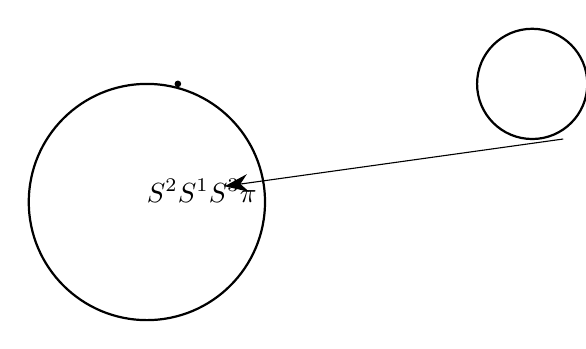
\begin{tikzpicture}[scale=1.0,every node/.style={font=\small}]
  % Base S^2
  \draw[thick] (0,0) circle (1.5);
   ode at (0,-2.0) {$S^2$};
  % Fiber circle S^1 above a base point
  \fill (0,1.5) circle (1.2pt);
  \draw[thick] (4.5,1.5) circle (0.7);
   ode at (4.5,2.6) {$S^1$ fiber};
  % Arrow indicating projection
  \draw[-{Stealth[length=3mm]}] (4.5,0.8) -- (0.2,0.2);
  % Total space S^3 label
   ode at (4.5,-2.0) {$S^3$};
  % Map labels
   ode at (2.4,0.9) {$\pi$};
\end{tikzpicture}
\caption{Hopf fibration $S^3 \xrightarrow{\ \pi\ } S^2$: each base point carries a circular fiber $S^1$.
The director $\mathbf n(q)=qKq^{-1}$ lives on $S^2$, while motion along the fiber encodes gauge time.}
\label{fig:hopf-schematic}
\end{figure}
\subsection[3.4. The ``quantum quaternion'' (placeholder)]{3.4. The ``quantum quaternion'' (placeholder)}
\label{subsec-3-4-the-quantum-quaternion-placeholder}

Here we only set notation: by ``quantum quaternion'' we mean the flow state endowed with a Hilbert-space structure over the complex slice $\mathrm{span}\{1,K\}$, suitable for spinor representations and Berry phases~\cite{Berry1984}. Full QM linkage is deferred to a separate paper.


% =============================================================
\section[Objects]{Objects}
\label{sec-objects}

 oindent\textit{Roadmap.} The next formulas fix notation and the geometric carriers we use throughout. 
In particular, the phase state $(\vartheta,\mathbf u)$ selects a complex slice 
$\mathbb C_{\mathbf u}\subset\mathbb H$; collinear compositions become ordinary circular sums on this slice, 
while non-collinear compositions generate a genuine 3D rotation (Wigner–Thomas) via quaternion multiplication.
This explains why we keep both $\vartheta$ and $\mathbf u$ as primary objects.

A fundamental particle is an elementary object with nonzero phase $\vec{\chi} eq0$. Composite objects are phase configurations; to represent them in phase space one may require additional dimensions, except for the photon, whose phase is always aligned with the imaginary axis:
\begin{equation}
\mathbf{p}=\frac{d\vec{\chi}}{d\chi_l}=p\,\mathbf{l}\in\Im.
\label{eq:31}
\end{equation}
Non-photonic phenomena are associated with nonzero real projection and nonzero mass. A complex object can be identified with an event or worldline; the photon corresponds to a null-interval point encoding information about the event.

Any object's phase can be rotated to the \emph{zero} (purely real) direction,
\begin{equation}
\vec{\chi}_0=R\in\Re.
\label{eq:32}
\end{equation}
An object $A$ moving with speed $v$ relative to a rest observer has
\begin{equation}
\vec{\chi}_A=R\,e^{\vartheta_A\mathbf{l}},\qquad
\sin\vartheta_A=\frac{v}{\mathtt{c}}\equiv\beta.
\label{eq:33}
\end{equation}

 oindent\textit{From unit norm to the interval.}
We will repeatedly use that $cd\tau= c\,dt\,cos\vartheta$ and $d\mathbf x=c\,dt\,sin\vartheta\,\mathbf u$.
Thus the identity $cos^{2}\vartheta+sin^{2}\vartheta=1$ is exactly the Minkowski metric statement 
$(cd\tau)^{2}=(cdt)^{2}-d\mathbf x^{2}$; from now on, square-root expressions are traded for circular 
trigonometry in $\vartheta$.


\subsection[Space as a symmetric phase pair]{Space as a symmetric phase pair}
\label{subsec-space-as-a-symmetric-phase-pair}

From \eqref{eq:14}, a naive zero-angle limit would remove the imaginary projection, contradicting observability. We enforce a nonvanishing spatial projection by pairing opposite-phase tilts:
\begin{equation}
\vec{\chi}^{\pm}=R\,e^{\pm\zeta\,\mathbf{l}},\qquad
\vec{\chi}_l:=\frac{\vec{\chi}^+-\vec{\chi}^-}{2}=R\,\mathbf{l}\sin\zeta,
\label{eq:311}
\end{equation}
where $\zeta$ is an \emph{internal angle} (intrinsic to the object; heuristically linked to mass/density). The local decomposition is
\begin{equation}
\vec{\chi}_0=\vec{\chi}_\tau+\vec{\chi}_l
=Rcos\zeta+R\,\mathbf{l}\sin\zeta,
\label{eq:312}
\end{equation}
with unit components (normalized by $R$): the real component is $cos\zeta$ and the imaginary component is $sin\zeta$.

\subsection[Absolute, local, and observed time]{Absolute, local, and observed time}
\label{subsec-absolute-local-and-observed-time}

Define \emph{absolute} time $t=t(\tilde{H})$ at the zero phase direction; it is the fastest clock and useful for normalization between different phase speeds. Along the local real direction,
\begin{equation}
dx_0=\frac{d}{d\chi}\Re(\vec{\chi})\,d\chi
=\frac{\vec{\chi}^+ + \vec{\chi}^-}{2}\,d\chi
=\cos\zeta\,d\chi
=:d\tau.
\label{eq:321}
\end{equation}
Here $d\chi_0:=cos\zeta\,d\chi$ is the projection of $d\chi$ onto the local real axis; in \cref{sec:norm} we calibrate $d\tau=(1/ u_0)\,d\chi_0$. The observed proper time of $A$ relative to the rest observer is
\begin{equation}
\tilde{H}_A=\Re\!\left(\frac{d\vec{\chi}_A}{d\vec{\chi}_0}\right)
=\cos\vartheta_A
=\sqrt{1-\sin^2\vartheta_A}
=\sqrt{1-\frac{v^2}{\mathtt{c}^2}}
=\frac{1}{\gamma}.
\label{eq:322}
\end{equation}

\subsection[Normalization]{Normalization}\label{sec:label}
 oindent\textit{Calibration.}
We fix the calibration by the observer’s clock and speed budget: 
$cos\vartheta \equiv d\tau/dt$ and $sin\vartheta \equiv \beta$.
This choice does not restrict generality: any overall rescaling of the underlying flow is absorbed into the 
definitions of $t$ and $c$, leaving all dimensionless observables unchanged.

Let local time be parameterized by \emph{phase}; introduce a reference frequency $ u_0$ and set
\begin{equation}
d\tau=\frac{1}{ u_0}\,d\chi_0.
\label{eq:331}
\end{equation}
By the chain rule,
\begin{equation}
dx_0=\tilde{H}\,d\chi
=\frac{dx_0}{d\chi_0}\frac{d\chi_0}{d\tau}\,d\tau
=\tilde{H}\,\dot{\chi}\,d\tau
=: \dot{H}\,d\tau,
\label{eq:332}
\end{equation}
where $ u:=d\chi/d\tau$, $\dot{\chi}:= u/ u_0$, and $\dot{H}:=\tilde{H}\,\dot{\chi}$. Choosing the calibration $\dot{H}\equiv \mathtt{c}$ gives $dx_0=\mathtt{c}\,d\tau$. Similarly for space,
\begin{equation}
dx_l=\tilde{L}\,d\chi
=\frac{dx_l}{d\chi_0}\frac{d\chi_0}{dl}\,dl
=\tilde{L}\,\chi'\,dl
=:L'\,dl,\qquad \chi':=\frac{d\chi}{dl}.
\label{eq:333}
\end{equation}
From $dx_0=dx_l$ for light one gets
\begin{equation}
\mathtt{c}=\tilde{L}'\,\frac{dl}{d\tau},
\label{eq:334}
\end{equation}
hence with temporal calibration to $\mathtt{c}$ the spatial scale becomes unit: $\tilde{L}'=1$.

\subsection[Light and $c]{Light and $\mathtt{c}$ as a calibration constant}
From the normalized forms,
\begin{equation}
\frac{\mathtt{c}}{\dot{\chi}}\,d\chi=\frac{1}{\chi'}\,d\chi
\quad\Rightarrow\quad
\mathtt{c}=\frac{\dot{\chi}}{\chi'}=\frac{dl}{d\tau},
\label{eq:341}
\end{equation}
i.e.\ $\mathtt{c}$ is a \emph{calibration constant} tying temporal and spatial measures, independent of local phase variation. Equation \eqref{eq:341} also reads
\begin{equation}
\mathtt{c}=\left(\frac{d\chi}{d\tau}\right)\!\left[\frac{dl}{d\chi}\right]\sim ( u)\,[\lambda],
\label{eq:343}
\end{equation}
matching frequency and wavelength of a photon, with $\chi$ as its phase. For a lightlike trajectory,
\begin{equation}
ds^2=\mathtt{c}^2\!\left(\frac{d\chi^2}{\dot{\chi}^2}-\frac{d\chi^2}{\dot{\chi}^2}\right)=0.
\label{eq:344}
\end{equation}
At unit frequency, $\tau=\chi$: the photon's ``proper time'' is its phase, and the length of its phase-speed vector equals its wavelength, $\tilde{H}_p=\lambda$. Finally, the kinematic slope in phase coordinates is
\begin{equation}
\frac{dx_l}{dx_0}
=\frac{\tilde{L}\,d\chi}{\tilde{H}\,d\chi}
=sin\vartheta
=\frac{v}{\mathtt{c}}
\equiv \beta,
\label{eq:345}
\end{equation}
so $\vartheta=\pi/2$ implies $v=\mathtt{c}$.

\subsection[Lorentz factor via reparameterization]{Lorentz factor via reparameterization}
A change of direction of the phase speed transforms
\begin{equation}
\tilde{H}^2=\tilde{S}^2+\tilde{L}^2 \;\longmapsto\;
\dot{H}^2=\dot{S}^2+\dot{L}^2.
\label{eq:351}
\end{equation}
\textbf{Lemma (parameter-change identity).} The transition $\tilde{H}\to\dot{S}$ is the manifestation of evolving phase speed under the parameter change $\chi\mapsto \tau(\chi)$, with local Jacobian
\begin{equation}
\frac{d\tau}{d\chi}=cos\zeta(\chi)cos\vartheta(\chi)
\quad\Rightarrow\quad
\mathcal{J}(\zeta,\vartheta):=\frac{d\chi}{d\tau}=\frac{1}{cos\zeta\,cos\vartheta}.
\label{eq:353}
\end{equation}
Then
\begin{equation}
\dot{H}=\tilde{H}\,\mathcal{J},\qquad \dot{L}=\tilde{L}\,\mathcal{J}.
\label{eq:354}
\end{equation}
In differential form,
\begin{equation}
d\ln\dot{H}=d\ln\mathcal{J}=\tan\zeta\,d\zeta+\tan\vartheta\,d\vartheta.
\label{eq:355}
\end{equation}
For a \emph{pure boost} ($d\zeta=0$) one has $d\dot{H}=\dot{H}\tan\vartheta\,d\vartheta$. Absorbing a constant $\cos\zeta$ into the calibration (set $\zeta=0$ henceforth), we obtain
\begin{equation}
\tilde{H}^2=\dot{H}^2-\dot{L}^2=\sec^2\vartheta\,(\tilde{H}^2-\tilde{L}^2)=\gamma^2(\tilde{H}^2-\tilde{L}^2).
\label{eq:356}
\end{equation}
\textbf{Corollary.} In phase space the Euclidean norm $\tilde{H}$ is conserved; in observed time the Minkowski norm $\dot{S}$ is conserved; they are identical as quantities:
\begin{equation}
\boxed{\ \tilde{H}=\dot{S}\ }.
\label{eq:357}
\end{equation}

\subsection[Rapidity and the phase angle]{Rapidity and the phase angle}
By definition,
\begin{equation}
\beta=\frac{v}{\mathtt{c}}=sin\vartheta,\qquad \tanh\eta=\beta,\qquad
d\eta=\frac{d\beta}{1-\beta^2}.
\label{eq:361}
\end{equation}
With $d\beta=\cos\vartheta\,d\vartheta$ and $1-\beta^2=\cos^2\vartheta$,
\begin{equation}
d\eta=\sec\vartheta\,d\vartheta,\qquad
\eta(\vartheta)=\int \sec\vartheta\,d\vartheta
=\ln|\sec\vartheta+\tan\vartheta|
=\tfrac12\ln\frac{|1+sin\vartheta|}{|1-sin\vartheta|}.
\label{eq:364}
\end{equation}
Fixing $\eta(0)=0$,
\begin{equation}
e^{\eta(\vartheta)}=\sqrt{\frac{1+sin\vartheta}{1-sin\vartheta}},\qquad
\gamma=\frac{1}{\sqrt{1-\beta^2}}=\sec\vartheta=cosh\eta.
\label{eq:365}
\end{equation}

\paragraph{Remark (groups).} Observables satisfy $\beta=\sin\vartheta=\tanh\eta$ and $\gamma=\sec\vartheta=\cosh\eta$. Thus Euclidean rotations in the phase circle (\,$U(1)$ with angle $\vartheta$\,) reproduce the numerical factors of hyperbolic boosts in $SO^+(1,1)$ (rapidity $\eta$) \emph{after} reparameterizing time. We do not claim an isomorphism $U(1)\cong SO(1,1)$; only the equality of observable combinations under the change of parameter.

\subsection[Velocity addition]{Velocity addition}
\label{sec:vel-addition}

\paragraph{Notation.}
In unimetry, an inertial boost is a \emph{D-rotation}
\begin{equation}
\label{eq:auto:32}
\mathcal{B}(\uhat,\psi):\quad \mathbf q \mapsto d\,\mathbf q\,d,
\qquad
d=cos\frac{\psi}{2}+\uhat\,sin\frac{\psi}{2},
\end{equation}
and a spatial rotation is an \emph{R-rotation}
\begin{equation}
\label{eq:auto:33}
\mathcal{R}(\hat{\mathbf n},\phi):\quad \mathbf q \mapsto r\,\mathbf q\,r^{-1},
\qquad
r=cos\frac{\phi}{2}+\hat{\mathbf n}\,sin\frac{\phi}{2}.
\end{equation}
Kinematic mapping: $\beta\equiv v/c=\sin\psi$, $\gamma=1/\cos\psi$,
$\displaystyle \tan\frac{\psi}{2}=\frac{\gamma\beta}{\gamma+1}$.
For quaternionic/GA accounts of rotors and Lorentz boosts see \cite{Hamilton1844,HestenesSobczyk1984,DoranLasenby2003}.

\subsubsection{Wigner rotation}\label{ssubsec-wigner-rotation}

\label{subsec:wigner}

Let $d_1,d_2$ be D-rotors of two successive boosts. The raw action on any unimetry 4-object is
\begin{equation}
\label{eq:auto:34}
\mathbf q' = d_2 d_1\, \mathbf q\, d_1 d_2 \equiv L_{12}\,\mathbf q\,L_{21},\qquad
L_{12}=d_2 d_1,\ \ L_{21}=d_1 d_2.
\end{equation}
Define $d_{12}$ to be the unique D-rotor reproducing the combined spatio--temporal tilt of $L_{12}$:
\begin{equation}
\boxed{\, d_{12}\,\mathbf e_t\, d_{12} \;=\; L_{12}\,\mathbf e_t\, L_{21},\qquad \Re(d_{12})\ge0 \,}
\label{eq:d12-uniqueness}
\end{equation}
(the sign choice removes the trivial two-fold ambiguity). Then the \emph{Wigner rotor} is the residual
R-rotation in the symmetric D--R factorization:
\begin{equation}
\boxed{\, L_{12}=d_{12}\,r_W,\qquad L_{21}=r_W^{-1}\,d_{12} \,}
\label{eq:DR-polar}
\end{equation}
equivalently,
\begin{equation}
\boxed{\, r_W=\bar d_{12}\,L_{12}=L_{21}\,\bar d_{12} \,}.
\label{eq:wigner-rotor-def}
\end{equation}
Hence the observed map after compensating the tilt is $\,\bar d_{12}\,\mathbf q'\,\bar d_{12}=r_W\,\mathbf q\,r_W^{-1}$.

\begin{figure}[!ht]
\centering
\begin{tikzpicture}[>=Latex, node distance=32mm]
   ode (q) {$\mathbf q$};
   ode (d1) [right=of q] {$d_1\,\mathbf q\,d_1$};
   ode (d2) [right=of d1] {$d_2 d_1\,\mathbf q\,d_1 d_2$};
   ode (rw) [below=20mm of d2] {$r_W\,\mathbf q\,r_W^{-1}$};
  \draw[->] (q) -- node[above] {$d_1$} (d1);
  \draw[->] (d1) -- node[above] {$d_2$} (d2);
  \draw[->] (d2) -- node[right] {$\bar d_{12}$ on both sides} (rw);
  \draw[->, dashed, bend left=12] (q) to node[above] {$d_{12}$} (d2);
\end{tikzpicture}
\caption{Two successive D-rotations (boosts) and compensation of the net spatio--temporal angle by the conjugate of $d_{12}$, leaving a pure R-rotation $r_W$.}
\label{fig:tikz-wigner-pullback}
\end{figure}

\subsubsection{Thomas precession}\label{ssubsec-thomas-precession}

\label{subsec:thomas}
The continuous limit of Wigner rotation for a time-dependent velocity direction $\uhat(t)$ yields
\begin{equation}
\label{eq:auto:38}
\boldsymbol{\omega}_T=(\gamma-1)\,\bigl(\uhat\times \dot{\uhat}\bigr)
=\frac{\gamma^2}{\gamma+1}\,\frac{\mathbf a\times \mathbf v}{c^2},\qquad
\gamma=\frac{1}{cos\psi}.
\end{equation}
For uniform circular motion ($|\mathbf v|=\mathrm{const}$) with $\dot{\uhat}=\boldsymbol{\Omega}\times\uhat$ one has
$\lvert\boldsymbol{\omega}_T\rvert=(\gamma-1)\,\Omega$.
\subsection[Doppler shift]{Doppler shift}
Define the observed frequency as the phase growth rate in the observer's proper time:
\begin{equation}
 u:=\frac{d\chi}{d\tau}.
\label{eq:381}
\end{equation}
For two successive wavefronts the phase increment is identical, hence
\begin{equation}
\frac{ u_{\mathrm{obs}}}{ u_{\mathrm{src}}}
=\frac{d\chi/d\tau_{\mathrm{obs}}}{d\chi/d\tau_{\mathrm{src}}}
=\frac{d\tau_{\mathrm{src}}}{d\tau_{\mathrm{obs}}}.
\label{eq:382}
\end{equation}
Longitudinal case: during $\gamma\,d\tau_{\mathrm{src}}$ in the observer frame the source displaces by $\pm v\,\gamma\,d\tau_{\mathrm{src}}$ (``$+$'' receding, ``$-$'' approaching). Then
\begin{equation}
d\tau_{\mathrm{obs}}=\gamma\,d\tau_{\mathrm{src}}(1\pm\beta),\qquad
\Rightarrow\quad
\boxed{\ \frac{ u_{\mathrm{obs}}}{ u_{\mathrm{src}}}=\frac{1}{\gamma(1\pm\beta)}\ }.
\label{eq:384}
\end{equation}
Equivalent forms (with $\beta=\sin\vartheta$, $\gamma=\sec\vartheta$ and rapidity $\eta$):
\begin{equation}
\frac{ u_{\mathrm{obs}}}{ u_{\mathrm{src}}}
=\sqrt{\frac{1\mp\beta}{1\pm\beta}}
=\sec\vartheta\,(1\mp\sin\vartheta)
=e^{\mp\eta}.
\label{eq:385}
\end{equation}
Transverse Doppler ($\phi=90^\circ$ in the observer's frame):
\begin{equation}
\frac{ u_{\mathrm{obs}}}{ u_{\mathrm{src}}}=\frac{1}{\gamma}=cos\vartheta.
\label{eq:389}
\end{equation}
General line-of-sight (LOS) angle $\phi$ in the observer's frame:
\begin{equation}
\boxed{\ \frac{ u_{\mathrm{obs}}}{ u_{\mathrm{src}}}=\gamma\,(1-\beta\cos\phi)\ }.
\label{eq:3810}
\end{equation}
Wavelength ratios are inverse to frequency ratios.

% === Gravity section (moved here) ===



% =============================================================
\section[Chapter 5. Optics]{Chapter 5. Optics}
\label{ch:optics}
We show that $\zeta$ is the refractive angle of the same flow:
\begin{equation}
  v_{\rm ph}(\zeta)=ccos\zeta,\qquad n(\zeta)=\frac{c}{v_{\rm ph}}=\sec\zeta,\qquad \varepsilon_{\rm flow}\mu_{\rm flow}=\frac{n^2}{c^2}=\frac{1}{c^2cos^2\zeta}.
\end{equation}
Fermat’s principle with $n(\mathbf x)=\sec\zeta(\mathbf x)$ yields Snell’s law and lensing. Frequency-independent $\zeta$ gives achromatic refraction; dispersion enters via $\zeta(\omega)$.


% =============================================================
\section[Chapter 6. Gravity as phase rotation]{Chapter 6. Gravity as phase rotation}
\label{ch:gravity}
\subsection[6.1. Normalization, tetrads, and the Rindler limit]{6.1. Normalization, tetrads, and the Rindler limit}
\label{subsec-6-1-normalization-tetrads-and-the-rindler-limit}

The statement “$\cos \vartheta \propto e^{(0)}{}_{\mu} u^{\mu}$” must be normalized. With an orthonormal tetrad $e^{(a)}{}_{\mu}$ and 4-velocity $u^{\mu}$, one has
\begin{equation}
  u^{(0)} = e^{(0)}{}_{\mu}u^{\mu} = \gamma c = \frac{c}{cos\vartheta}\quad\Rightarrow\quad \boxed{\;cos\vartheta = \frac{c}{e^{(0)}{}_{\mu}u^{\mu}}\;}. 
\end{equation}
In a stationary weak field, a gravitational tilt $\phi$ modifies local rates as $d\tau/dt=\cos\phi$, reproducing clock redshift and Shapiro-like delays~\cite{Shapiro1964} via an effective index $n_g=\sec\phi$. The Rindler limit is recovered by a linear potential: constant proper acceleration corresponds to a constant gradient of $\phi$, with optical metric $ds^2_{\rm opt}=dt^2-n_g^2 d\ell^2$.

\subsection[6.2. Local conservation and Friedmann-like effects]{6.2. Local conservation and Friedmann-like effects}
\label{subsec-6-2-local-conservation-and-friedmann-like-effects}

In unimetry, local energy--momentum conservation is encoded as $dJ_E=0$ with $J_E=\star(\kappa\alpha)$. For a comoving domain with no exchange ($\dot\kappa=0$) and stationary $\mathbf n$, the intrinsic tilt $\zeta$ is constant along streamlines ($\dot\zeta=0$). Conversely, evolution of $\zeta$ produces Friedmann-like effects for waves carried by the same flow:
\begin{equation}
  \omega(t)=\frac{c}{a(t)\,n(t)}k_{\rm com}\;\Rightarrow\;1+z=\frac{a_0 n_0}{a_{\rm em}n_{\rm em}},\qquad n=\sec\zeta.
\end{equation}
Thus, changes in $\zeta$ at fixed scale $a$ generate additional (achromatic) redshifts and time dilations beyond pure expansion.


% =============================================================
\section[Chapter 7. Discussion]{Chapter 7. Discussion}
\label{ch:discussion}
\textbf{Scope and limits.} We deliberately keep full GR field equations and quantum measurement out of Part I. The present model treats gravity as a phase-tilt field ($\phi$) and optics/clock rates as consequences of the same geometry.

\textbf{Testable consequences.}
\begin{itemize}
  \item \emph{SR on a circle:} collider kinematics can be implemented with circular identities ($\beta=\sin\vartheta$, $\gamma=\sec\vartheta$), simplifying composition and Doppler chains.
  \item \emph{Optical tilt:} refractive index of a flow is $n=\sec\zeta$. Spatial gradients $ abla\zeta$ bend rays; temporal drifts $\dot\zeta$ create achromatic frequency shifts.   \item \emph{Wigner residue:} two D-tilts yield a net spatial rotation about $V_2\times V_1$ with angle matching the standard Wigner formula.
  \item \emph{Cosmological factorization:} $(1+z)=(a_0/a_{\rm em})(n_0/n_{\rm em})$, enabling disentangling expansion from intrinsic tilt evolution.
\end{itemize}

\textbf{Computational advantage (colliders).} Quaternion D-tilts avoid explicit 4×4 Lorentz matrices and hyperbolic functions in compositions. For repeated non-collinear boosts, accumulating a single unit quaternion per step reduces memory traffic and floating-point ops; composing $N$ boosts is $O(N)$ quaternion multiplies (each $\approx 16$ mult + 12 add), while matrix re-normalization and re-orthogonalization are avoided. See Appendix for a crude operation count and pseudo-code.


% =============================================================
\section[Chapter 8. Conclusion]{Chapter 8. Conclusion}
\label{ch:conclusion}
We presented a unified flow picture where a single intrinsic angle $\zeta$ controls SR time-rate, optical speed, and refractive response; an external gravitational angle $\phi$ accounts for weak-field clock and light effects; and a kinematic angle $\vartheta$ reparametrizes SR on a circle. Dynamics follows from the curl of the director $\mathbf n$ with $\mathbf F=E\, abla\times\mathbf n$ and mass $m=\kappa c$. The quaternion--Hopf structure provides the native geometry; Wigner rotations emerge from non-commuting D-tilts. Part~II will connect this framework to quantum mechanics (spinors, Berry phases, and measurement), and to stronger-field gravitation.


% =============================================================
\appendix
\section*{Appendix. Wigner rotation equivalence and accounting}
\label{sec-appendix-wigner-rotation-equivalence-and-accounting}

\subsection*{A.1. Equivalence (kept as is)}
\label{subsec-a-1-equivalence-kept-as-is}

Successive D-tilts along $V_1,V_2\perp K$ compose to a net rotation (Wigner~\cite{Wigner1939}) about $V_2\times V_1$ with angle
\begin{equation}
  \tan\frac{\psi}{2}=\frac{sinh\frac{\eta_1}{2}\,sinh\frac{\eta_2}{2}\,sin\theta}{cosh\frac{\eta_1}{2}\,cosh\frac{\eta_2}{2}+sinh\frac{\eta_1}{2}\,sinh\frac{\eta_2}{2}\,cos\theta},\qquad \tanh\eta_i=sin\vartheta_i.
\end{equation}
This matches the standard Wigner rotation formula.

\subsection*{A.2. Counting advantage (crude)}
\label{subsec-a-2-counting-advantage-crude}

\textit{Setup.} Compose $N$ non-collinear boosts. Standard 4×4 Lorentz chaining uses per step roughly: one matrix build ($\sim20$ flops including trig/hyperbolic), one $4\times4\times4$ multiply ($64$ mult + $48$ add), plus re-normalization. Quaternion D-tilts store a unit quaternion per step and compose with one quaternion multiply ($16$ mult + $12$ add); normalization is one scalar division per $\sim$few steps.

\textit{Result.} For large $N$, total ops drop by a factor $\sim 3$–$5$ and memory traffic halves, while numerical orthogonality is maintained by unit-norm enforcement. In collider tracking this yields fewer cache misses and simpler pipelines. (Exact factors depend on implementation and vectorization.)



% =============================================================
\section*{References}
\label{sec-references}

\begin{thebibliography}{99}
\bibitem{Hopf1931}
H.~Hopf, ``Über die Abbildungen der dreidimensionalen Sphäre auf die Kugelfläche,'' \emph{Mathematische Annalen} \textbf{104} (1931) 637--665. \href{https://doi.org/10.1007/BF01457962}{doi:10.1007/BF01457962}.

\bibitem{Thomas1926}
L.~H.~Thomas, ``The Motion of the Spinning Electron,'' \emph{Nature} \textbf{117} (1926) 514. \href{https://doi.org/10.1038/117514a0}{doi:10.1038/117514a0}.

\bibitem{Wigner1939}
E.~P.~Wigner, ``On Unitary Representations of the Inhomogeneous Lorentz Group,'' \emph{Annals of Mathematics} \textbf{40} (1939) 149--204. \href{https://doi.org/10.2307/1968551}{doi:10.2307/1968551}.

\bibitem{Berry1984}
M.~V.~Berry, ``Quantal phase factors accompanying adiabatic changes,'' \emph{Proceedings of the Royal Society A} \textbf{392} (1984) 45--57. \href{https://doi.org/10.1098/rspa.1984.0023}{doi:10.1098/rspa.1984.0023}.

\bibitem{Shapiro1964}
I.~I.~Shapiro, ``Fourth Test of General Relativity,'' \emph{Phys. Rev. Lett.} \textbf{13} (1964) 789--791. \href{https://doi.org/10.1103/PhysRevLett.13.789}{doi:10.1103/PhysRevLett.13.789}.

\bibitem{RindlerBook}
W.~Rindler, \emph{Relativity: Special, General, and Cosmological}, 2nd ed., Oxford University Press, 2006.

\bibitem{MTW}
C.~W.~Misner, K.~S.~Thorne, J.~A.~Wheeler, \emph{Gravitation}, W.~H.~Freeman, 1973.

\bibitem{Jackson}
J.~D.~Jackson, \emph{Classical Electrodynamics}, 3rd ed., Wiley, 1999.
\end{thebibliography}

\end{document}
